

\actTitle{Worksheet 1.6A}



\noindent \textbf{Instructions:} Work together in groups of 3 or 4 to
complete the following problems.  You may be asked to share some of
your solutions on the board.


\noindent
Student goals:
  \begin{itemize}
  \item Determine the algebraic formula of a basic function given a
    written description or a graphical representation.
  \item Determine the algebraic formula for a function after a vertical translation or scaling.
  \item Determine the algebraic formula for a function after a
    horizontal translation or scaling.
  \item Determine the algebraic formula for a function after a vertical reflection.
  \end{itemize}


\begin{enumerate}
\item Graph the given function and determine how many points need to be plotted to understand the shape of the graph.

\begin{enumerate}
\item $f(x)=-3$, Number of points necessary to plot:  \underline{\phantom{alphabetsoup}}\\
 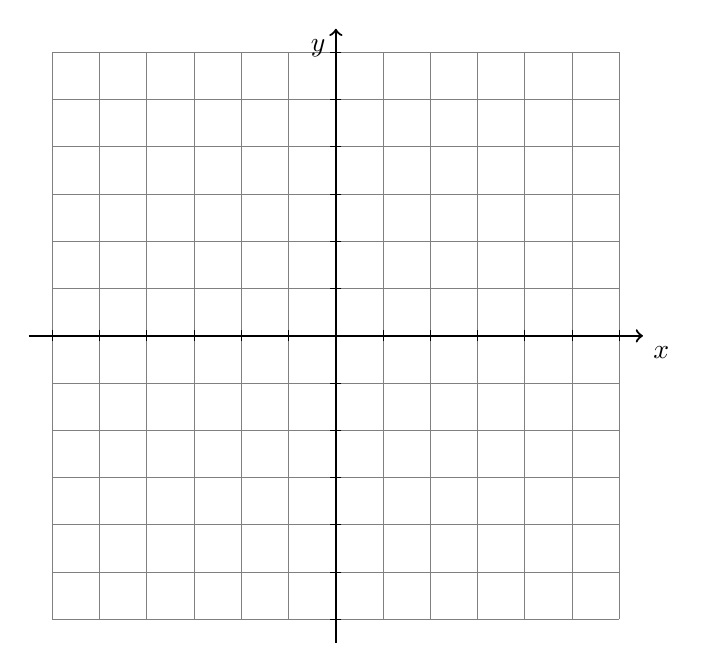
\begin{tikzpicture}[y=.6cm, x=0.6cm,font=\sffamily]
    %% ticks
    \draw[step = 1, gray] (-6,-6) grid (6,6);
    %% axis
    \draw[thick,->] (-6.5,0) -- coordinate (x axis mid) (6.5,0) node[anchor = north west] {$x$};
    \draw[thick,->] (0,-6.5) -- coordinate (y axis mid) (0,6.5) node[anchor = north east] {$y$};
    \foreach \y in {-6,-5,...,-1,1,2,...,6} {
      \draw (2pt, \y) -- (-2pt, \y);
    }
    \foreach \x in {-6,-5,...,-1,1,2,...,6} {
      \draw (\x,2pt) -- (\x,-2pt);
    }

  \end{tikzpicture}

\clearpage  

\item $m(x)=\sqrt[3]{x}$, Number of points necessary to plot:  \underline{\phantom{alphabetsoup}}\\
 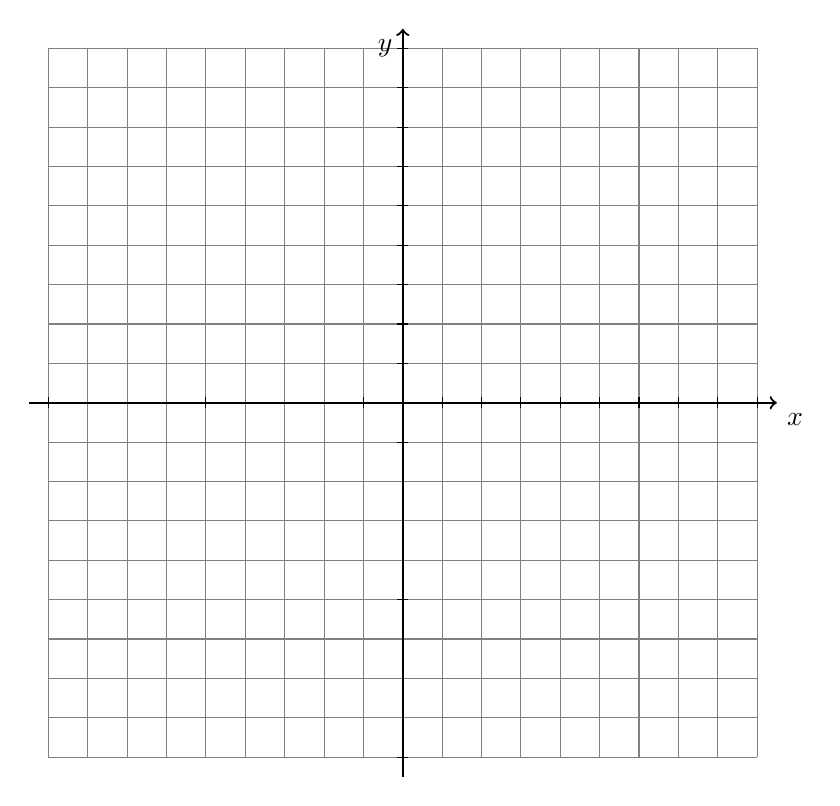
\begin{tikzpicture}[y=.5cm, x=.5cm,font=\sffamily]
    %% ticks
    \draw[step = 1, gray] (-9,-9) grid (9,9);
    %% axis
    \draw[thick,->] (-9.5,0) -- coordinate (x axis mid) (9.5,0) node[anchor = north west] {$x$};
    \draw[thick,->] (0,-9.5) -- coordinate (y axis mid) (0,9.5) node[anchor = north east] {$y$};
    \foreach \y in {-9,-5,...,-1,1,2,...,9} {
      \draw (2pt, \y) -- (-2pt, \y);
    }
    \foreach \x in {-9,-5,...,-1,1,2,...,9} {
      \draw (\x,2pt) -- (\x,-2pt);
    }

  \end{tikzpicture}
\vfill

\item $\displaystyle p(x)=\frac{1}{x}$, Number of points necessary to plot:  \underline{\phantom{alphabetsoup}}\\
 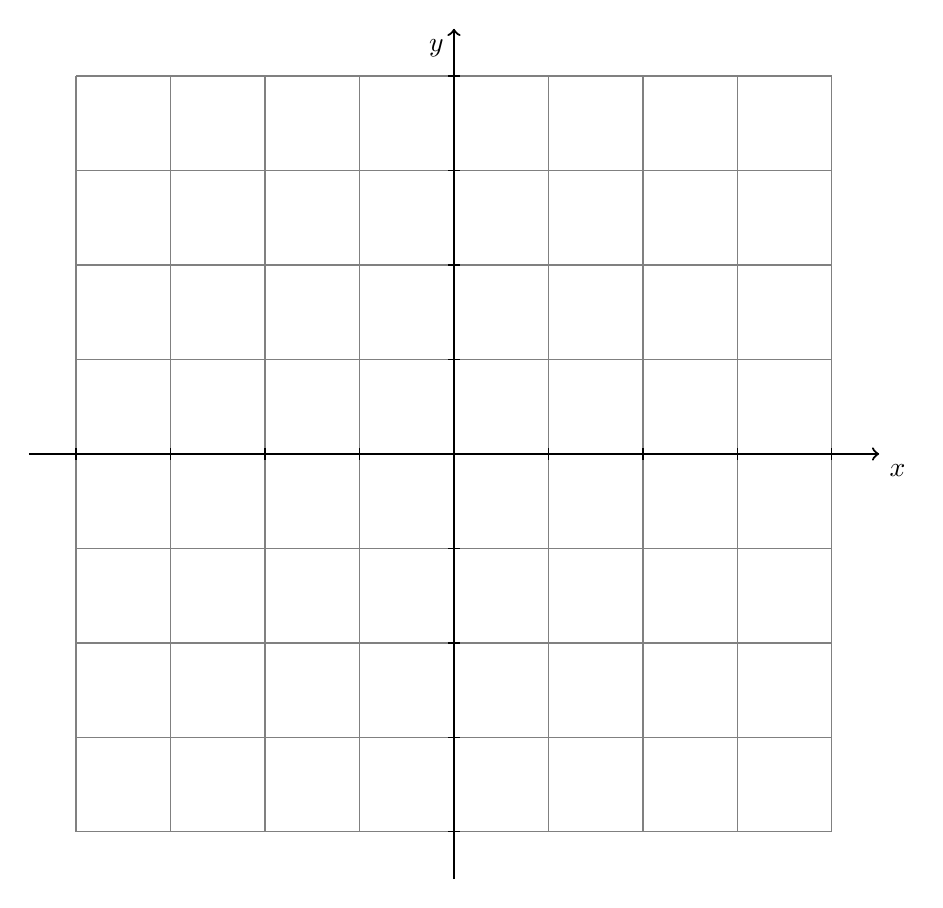
\begin{tikzpicture}[y=1.2cm, x=1.2cm,font=\sffamily]
    %% ticks
    \draw[step = 1, gray] (-4,-4) grid (4,4);
    %% axis
    \draw[thick,->] (-4.5,0) -- coordinate (x axis mid) (4.5,0) node[anchor = north west] {$x$};
    \draw[thick,->] (0,-4.5) -- coordinate (y axis mid) (0,4.5) node[anchor = north east] {$y$};
    \foreach \y in {-4,...,-1,1,2,...,4} {
      \draw (2pt, \y) -- (-2pt, \y);
    }
    \foreach \x in {-4,...,-1,1,2,...,4} {
      \draw (\x,2pt) -- (\x,-2pt);
    }

  \end{tikzpicture}


\end{enumerate}

\clearpage

\item  For this problem, let $q(x)=x^3$.

\begin{enumerate}
\item Graph $q(x)=x^3$.  Then determine the domain and range of $q(x)$.\\
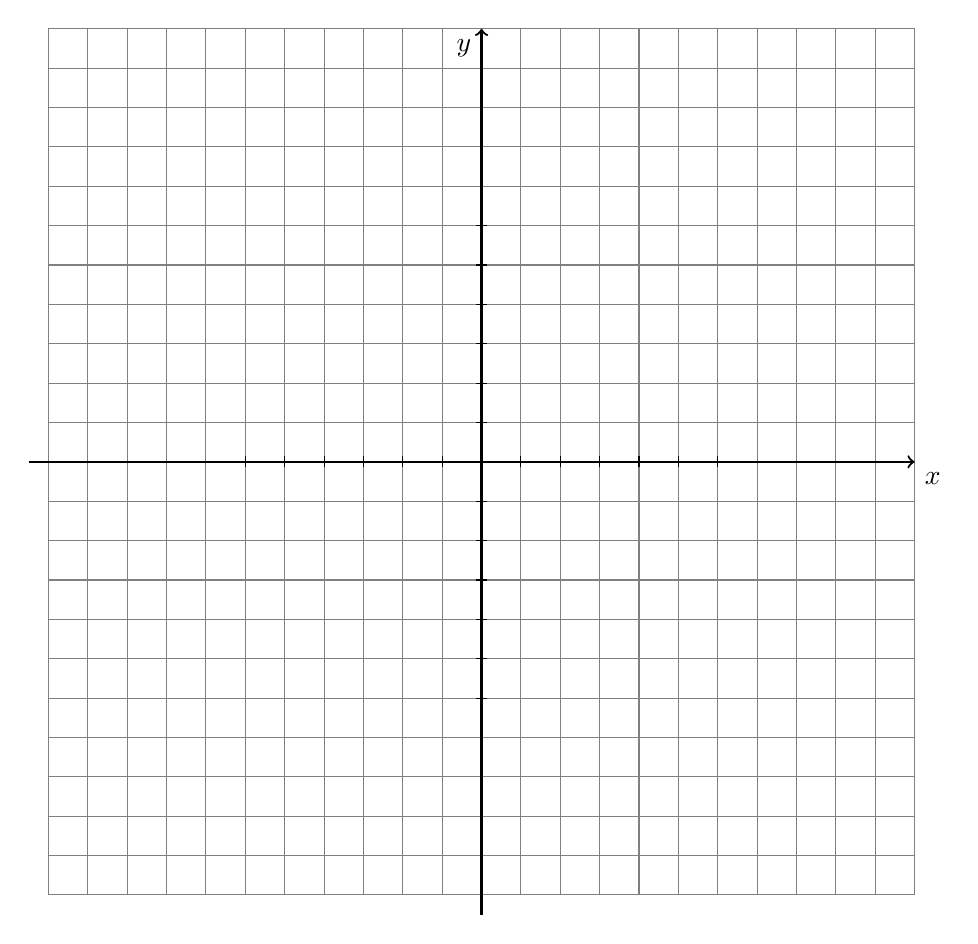
\begin{tikzpicture}[y=.5cm, x=0.5cm,font=\sffamily]
    %% ticks
    \draw[step = 1, gray] (-11,-11) grid (11,11);
    %% axis
    \draw[thick,->] (-11.5,0) -- coordinate (x axis mid) (11,0) node[anchor = north west] {$x$};
    \draw[thick,->] (0,-11.5) -- coordinate (y axis mid) (0,11) node[anchor = north east] {$y$};
    \foreach \y in {-6,-5,...,-1,1,2,...,6} {
      \draw (2pt, \y) -- (-2pt, \y);
    }
    \foreach \x in {-6,-5,...,-1,1,2,...,6} {
      \draw (\x,2pt) -- (\x,-2pt);
    }

  \end{tikzpicture}

\item Use part (a) to graph $r(x)=x^3+2$ above.  Then determine the domain and range of $r(x)$.
\vfill
\item Use part (a) to graph $s(x)=(x-2)^3$ above.  Then determine the domain and range of $s(x)$.
\vfill
\item Use part (a) to graph $u(x)=(x-2)^3+2$ above.  Then determine the domain and range of $u(x)$.
\vfill
\end{enumerate}




\newpage

\item  For this problem, let $q(x)=\sqrt{x}$.

\begin{enumerate}
\item Graph $q(x)=\sqrt{x}$.  Then determine the domain and range of $q(x)$.\\
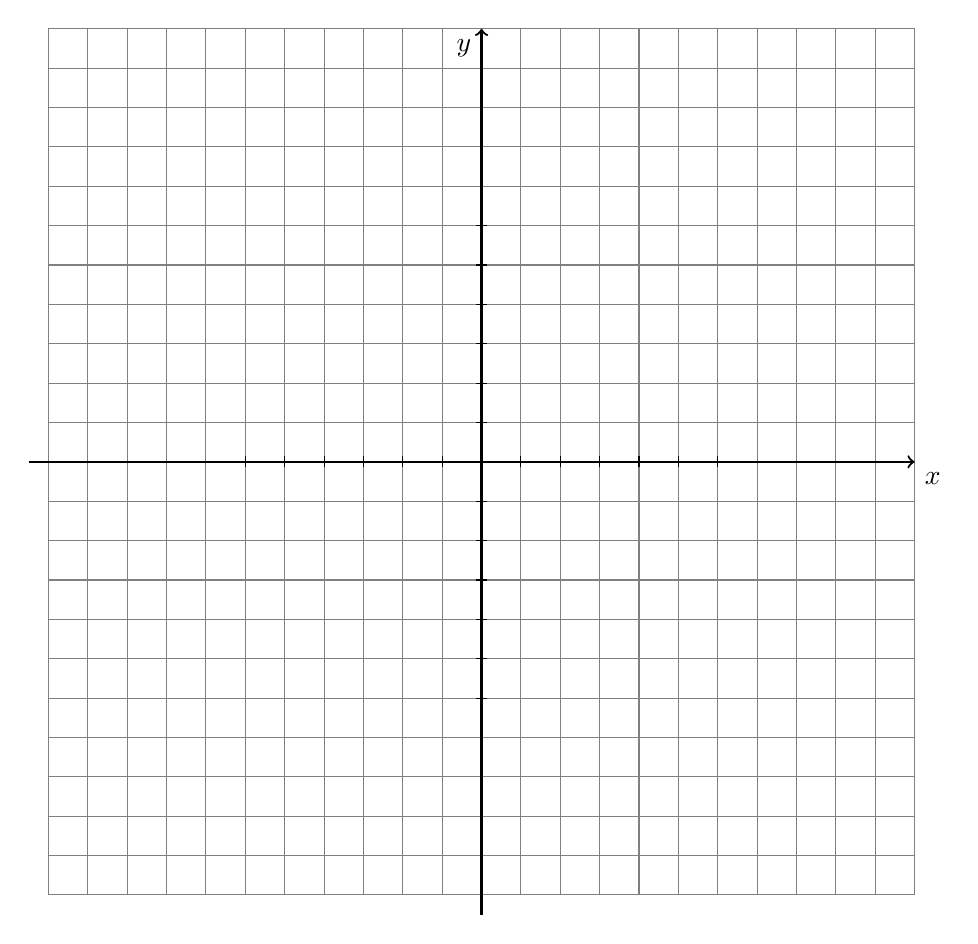
\begin{tikzpicture}[y=.5cm, x=0.5cm,font=\sffamily]
    %% ticks
    \draw[step = 1, gray] (-11,-11) grid (11,11);
    %% axis
    \draw[thick,->] (-11.5,0) -- coordinate (x axis mid) (11,0) node[anchor = north west] {$x$};
    \draw[thick,->] (0,-11.5) -- coordinate (y axis mid) (0,11) node[anchor = north east] {$y$};
    \foreach \y in {-6,-5,...,-1,1,2,...,6} {
      \draw (2pt, \y) -- (-2pt, \y);
    }
    \foreach \x in {-6,-5,...,-1,1,2,...,6} {
      \draw (\x,2pt) -- (\x,-2pt);
    }

  \end{tikzpicture}

\item Use part (a) to graph $r(x)=\sqrt{x}-5$ above.  Then determine the domain and range of $r(x)$.
\vfill
\item Use part (a) to graph $s(x)=\sqrt{x-1}$ above.  Then determine the domain and range of $s(x)$.
\vfill
\item Use part (a) to graph $u(x)=\sqrt{x-1}-5$ above.  Then determine the domain and range of $u(x)$.
\vfill
\end{enumerate}


\newpage

\item In words, explain how the graph of $f(x)=|x-4|+37$ is different from the graph of $g(x)=|x|$.
\vfill

\item Write an equation for the function that has been transformed.
\begin{enumerate}
\item $f(x)$ looks like $g(x)=x^2$ after it has been transformed by shifting 3 units to the right and 4 units up.  Write the equation of $f(x)$.
\vfill
\item $f(x)$ looks like $g(x)=\sqrt{x}$ after it has been transformed by shifting 5 units to the left and 1 unit down.  Write the equation of $f(x)$.
\vfill
\item $f(x)$ looks like $\displaystyle g(x)=\frac{1}{x}$ after it has been transformed by shifting 2 units to the left and 5 units up.  Write the equation of $f(x)$.
\vfill
\end{enumerate}

\item If the point $(-2,5)$ is on the graph of $y=f(x)$, find the corresponding point on the graph of $y=f(x+2)-4$
\vfill


\end{enumerate}

%
%\newpage
%
%\begin{center}
%	\begin{tikzpicture}[y=1.25cm, x=1.25cm,font=\sffamily,
%	mydot/.style={
%    circle,
%    fill=white,
%    draw,
%    outer sep=0pt,
%    inner sep=1.5pt
%  }]
%    %% Add a grid
%    \draw[step = 1, gray, very thin,opacity=0.85] (-6, -6) grid (6, 6);
% 	%% Draw the axes
%	\draw[thick,<->] (-6.5,0) -- coordinate (x axis mid) (6.5,0) node[anchor = north west] {$x$};
%    \draw[thick,<->] (0,-6.5) -- coordinate (y axis mid) (0,6.5) node[anchor = south west] {$y$};
%    %% Label the y axis
%    \foreach \y in {-6,...,-1,1,2,...,6} {
%      \draw (1pt, \y) -- (-1pt, \y) node[anchor = south east] {$\y$};
%    }
%    %% Label the x axis
%    \foreach \x in {-6,...,-1,1,2,...,6} {
%      \draw (\x,1pt) -- (\x,-1pt) node[anchor = north] {$\x$};
%    }
%    %% Draw the function.
%    \begin{scope}
%         \draw[very thick,black] (-3,2) -- (1,1);
%         \draw[very thick,black] (3.05,1.05) -- (4,3);
%    %semi-circle
%         \draw[very thick, black] (1,1) arc [radius=1, start angle=180, end angle= 5];
%     %parabola
%     %    \draw[ultra thick, black, domain=-5:0] plot (\x, {(-0.2)*(\x-5)*(\x+5)});
%     %dots
%         \fill[black] (-3, 2) circle[radius=0.5ex];
%         \fill[black] (1,1) circle[radius=0.5ex];
%         \fill[black] (4,3) circle[radius=0.5ex];
%         \draw[very thick, black] (3,1) circle[radius=0.5ex];
%
%
%    \end{scope}
%
%    %%\node[above=0.1cm] at (-2,2 )   {\nextXValue};
%
%  \end{tikzpicture}
%\end{center}


